\documentclass{article}
\usepackage{caption}
\usepackage{amssymb}
\usepackage{array}
\usepackage{geometry}
\usepackage{scrextend}
\usepackage{amsmath}
\usepackage{hyperref}
\usepackage{graphicx}
\usepackage{pdfpages}
\usepackage{multicol}

\title{EE102 Homework 1}
\author{Jacob Guenther}

\geometry{
	a4paper,
	total={170mm,257mm},
	left=20mm,
	top=20mm,
}

\newcommand{\problemstatement}[3]{
\noindent
\begin{tabular}{ m{0.5cm} m{42em} m{0.5cm} }
	({#1}) & {#2} & {#3}pts
\end{tabular}
}

\begin{document}

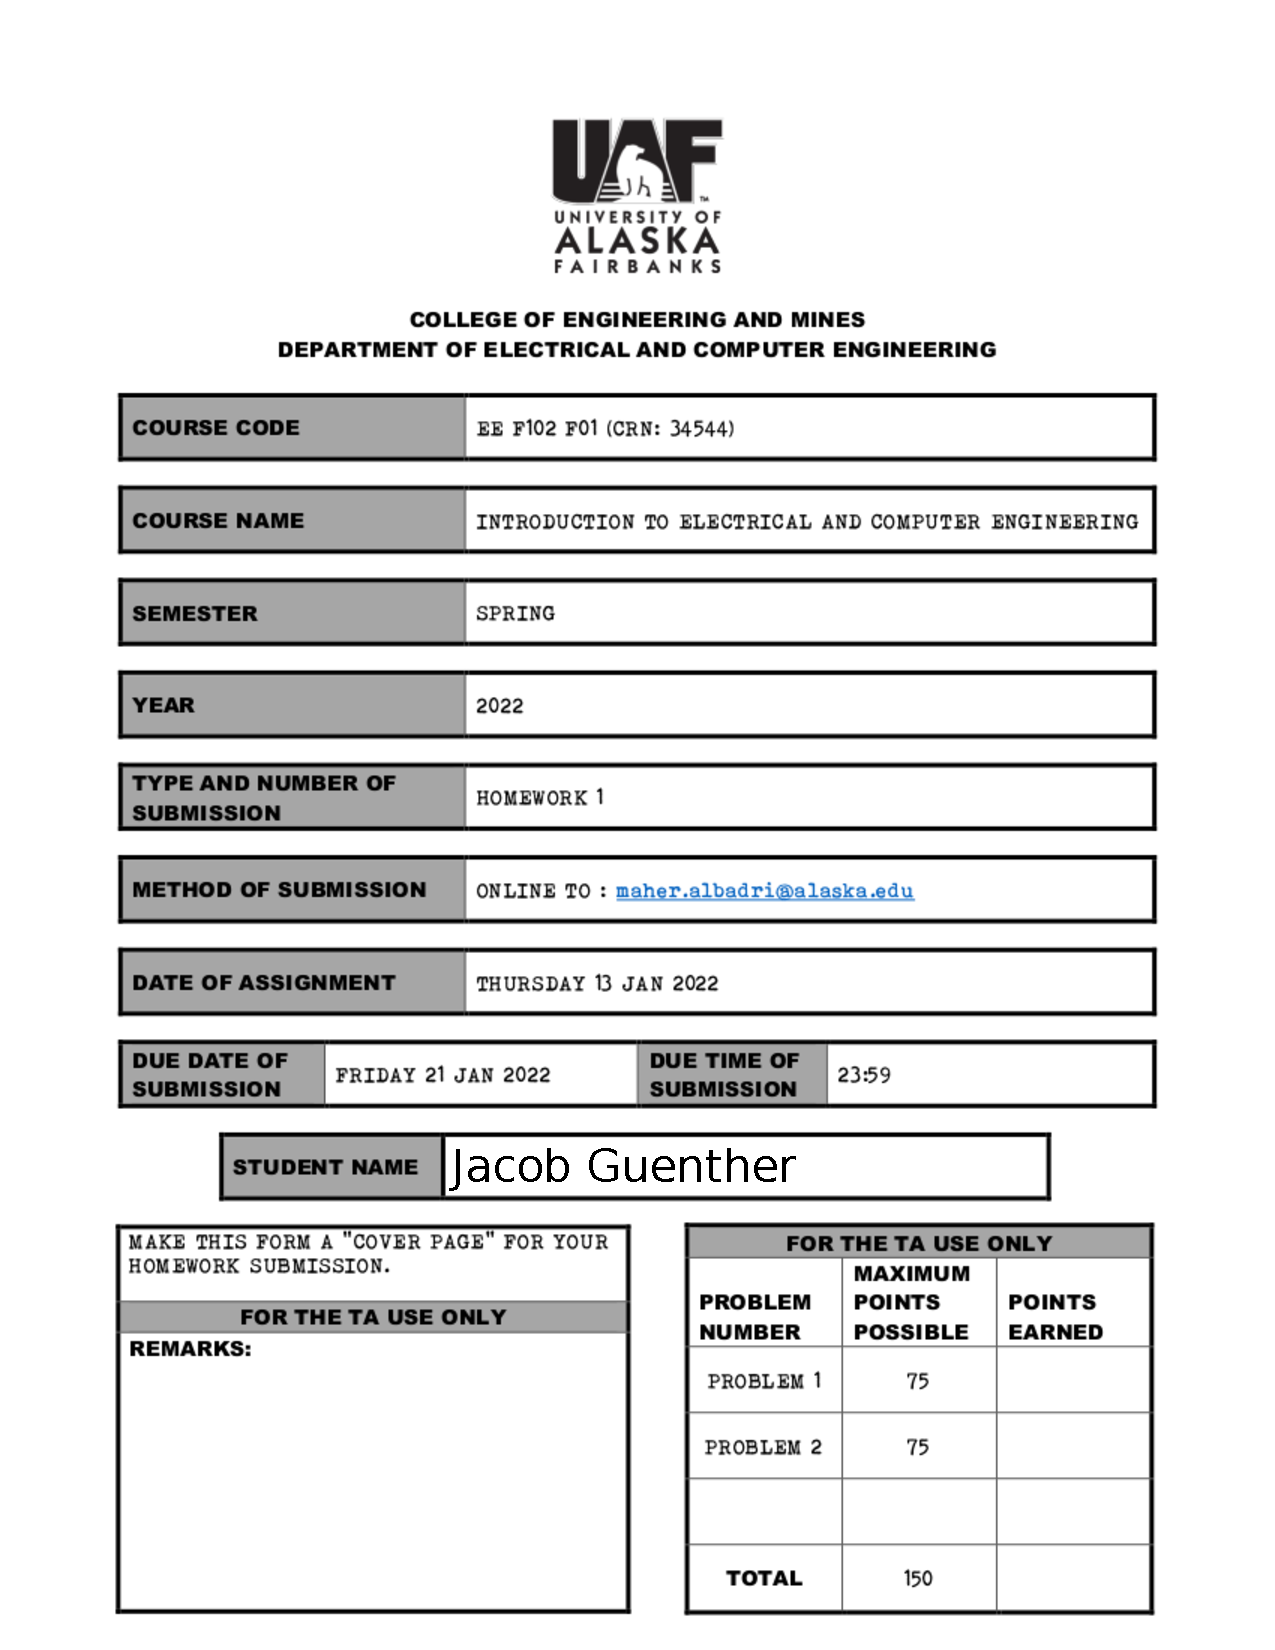
\includepdf[pages=1,pagecommand={}]{HW1cover.pdf}

\section{Problem HW-1-1}
\problemstatement{a}{500 N force is used to move an object over a distance of 1000 cm. Calculate the energy, in kJ, required to do this work.}{15}
\begin{addmargin}[1.5cm]{0em}
	\noindent
	\textbf{Note:}
	\begin{equation}
	1 \text{m} = 100 \text{cm}
	\end{equation}
	\begin{equation}
	\text{J} = \text{N} \cdot \text{m}
	\end{equation}
	\begin{equation}
	1 \text{kJ} = 1000 \text{J}
	\end{equation}
	\noindent
	\textbf{Solution:} \\
	Convert cm to m using equation (1).
	\[1000 \text{cm} \cdot {1 \text{m} \over 100 \text{cm}} = 10 \text{m}\]
	Calculate energy in J using equation (2).
	\[500 \text{N} \cdot 10 \text{m} = 5000 \text{J} \]
	Convert J to kJ using equation (3).
	\[5000 \text{J} \cdot {1 \text{kJ} \over 1000 \text{J}} = 5 \text{kJ} \] \\
	\noindent
	\textbf{Answer:} The energy required to move the object is \textbf{5kJ}. \\ \\
\end{addmargin}

\newpage
\problemstatement{b}{5kJ of energy is utilized to move an object a distance of 10 m. Calculate the applied force, in newtons (N).}{15}
\begin{addmargin}[1.5cm]{0em}
	\noindent
	\textbf{Solution:} \\
	Convert kJ to J using equation (3).
	\[5 \text{kJ} \cdot {1000 \text{J} \over 1 \text{kJ}} = 5000 \text{J} \]
	Calculate force in N using equation (2).
	\[{5000 \text{J} / 10 \text{m}} = 500 \text{N} \]
	\noindent
	\textbf{Answer:} The force applied to the object is \textbf{500N}. \\ \\
\end{addmargin}

\newpage
\problemstatement{c}{How many significant digits are in the following numbers:}{15}
% \: - medium space
\begin{enumerate}
	\item \(69.00056\:\text{m}\)
	\item \(0.01225600\:\text{ft}\)
	\item \(123.80000\:\text{in}\)
	\item \(1.0 \times 10^2\:\text{J}\)
\end{enumerate}
\begin{addmargin}[1.5cm]{0em}
	\noindent
	\textbf{Note:}
	\begin{itemize}
		\item All non-zero digits (1-9) are significant[1].
		\item Zeros that have any non zero digit anywhere to the left of them are considered significant zeros[1].
		\item All other zeros are not considered significant[1].
	\end{itemize}
	\noindent
	\textbf{Answer}
	\begin{enumerate}
		\item \(69.00056\:\text{m}\) has \textbf{7} significant digits. All of the digits are significant.
		\item \(0.01225600\:\text{ft}\) has \textbf{7} significant digits. The two leading zeros are not significant.
		\item \(123.80000\:\text{in}\) has \textbf{8} significant digits. All of the digits are significant.
		\item \(1.0 \times 10^2\:\text{J}\) has \textbf{2} significant digits. Both digits are significant.
	\end{enumerate}
\end{addmargin}

\newpage
\problemstatement{d}{Three methods were used to measure a 5 $\Omega$ resistor. Each measurement was repeated 4 times and tabulated in the following table. Determine the method with the highest accuracy. You can use a spreadsheet tool to perform quick calculations.}{15}
\begin{addmargin}[1.5cm]{0em}
	\begin{center}
	\captionof{table}{Measured Values\label{Tab:Tcr}}
	\begin{tabular}{| w{c}{2cm} | w{c}{2cm} | w{c}{2cm} |}
			\hline
			Method I ($\Omega$) & Method II ($\Omega$) & Method III ($\Omega$) \\ \hline
			5.0041 & 5.0022 & 5.1012 \\ \hline
			5.0151 & 5.0011 & 5.1112 \\ \hline
			5.0991 & 5.0101 & 5.1023 \\ \hline
			5.0261 & 5.0041 & 5.1022 \\ \hline
		\end{tabular}
	\end{center}	
	\noindent
	\textbf{Note:}
	\begin{equation}
		\text{absolute error} = \lvert x - x_i \rvert
	\end{equation}
	\noindent
	\textbf{Solution:}
	\begin{center}
		\captionof{table}{Absolute error using equation (4)\label{Tab:Tcr}}
		\begin{tabular}{| w{c}{2cm} | w{c}{2cm} | w{c}{2cm} | w{c}{2cm} |}
			\hline
			& Method I ($\Omega$) & Method II ($\Omega$) & Method III ($\Omega$) \\ \hline
			sample 1 & 0.14440 & 0.00220 & 0.10120 \\ \hline
			sample 2 & 0.01510 & 0.00110 & 0.11120 \\ \hline
			sample 3 & 0.09910 & 0.01010 & 0.10230 \\ \hline
			sample 4 & 0.02610 & 0.00410 & 0.10220 \\ \hline
			total error & 0.14440 & 0.01750 & 0.41690 \\ \hline
		\end{tabular}
	\end{center}
	\noindent
	\textbf{Answer:} Method II has the smallest absolute error so method II is the most accurate. \\
\end{addmargin}

\newpage
\problemstatement{e}{In the previous problem, determine which method has the highest precision.}{15}
\begin{addmargin}[1.5cm]{0em}
	\noindent
	\textbf{Note:}
	\begin{equation}
		\text{range} = x_{max} - x_{min}
	\end{equation}
	Mean
	\begin{equation}
		\mu = {\Sigma x_i \over N}
	\end{equation}
	Deviation
	\begin{equation}
		\text{deviation} = (x_i - \mu)^2
	\end{equation}
	Sample variance
	\begin{equation}
		\sigma^2 = { 1 \over {N - 1}} \Sigma (x_i - \mu)^2
	\end{equation}
	Sample standard deviation
	\begin{equation}
		\sigma = \sqrt{\sigma^2}
	\end{equation}
	\url{https://en.wikipedia.org/wiki/Standard_deviation}\\
	\noindent
	\textbf{Solution:}
	\begin{center}
		\captionof{table}{Range using equation (5)\label{Tab:Tcr}}
		\begin{tabular}{| w{c}{2cm} | w{c}{2cm} | w{c}{2cm} | w{c}{2cm} |}
			\hline
			& Method I ($\Omega$) & Method II ($\Omega$) & Method III ($\Omega$) \\ \hline
			min & 5.0041 & 5.0011 & 5.1012 \\ \hline
			max & 5.0991 & 5.0101 & 5.1112 \\ \hline
			range & 0.095 & 0.009 & 0.01 \\ \hline
		\end{tabular}
	\end{center}
	We can also use sample variance or sample standard deviation to measure precision. \\
	To calculate standard deviation first calculate the mean.
	\begin{align*}
		\mu_I &= { 5.0041 + 5.0151 + 5.0991 + 5.0261 \over 4}\\
		      &= 5.0361\\
		\mu_{II} &= { 5.0022 + 5.0011 + 5.0101 + 5.0041 \over 4}\\
		      &= 5.004375\\
		\mu_{III} &= { 5.1012 + 5.1112 + 5.1023 + 5.1022 \over 4}\\
		      &= 5.004375
	\end{align*}
	\begin{center}
		\captionof{table}{Standard deviation using equations (7), (8), and (9)\label{Tab:Tcr}}
		\begin{tabular}{| w{c}{4cm} | w{c}{2cm} | w{c}{2cm} | w{c}{2cm} |}
			\hline
			& Method I & Method II & Method III \\ \hline
			sample 1 deviation & 0.001024  & 4.7306E-06 & 9.1506E-06 \\ \hline
			sample 2 deviation & 0.000441  & 1.0726E-05 & 4.8651E-05 \\ \hline
			sample 3 deviation & 0.003969  & 3.2776E-05 & 3.7056E-06 \\ \hline
			sample 3 deviation & 0.0001    & 7.5625E-08 & 4.1006E-06 \\ \hline
			sample variance    & 0.0018447 & 1.6103E-05 & 2.1869E-05 \\ \hline
			sample standard deviation & 0.042950 & 0.0040128 & 0.0046764 \\ \hline
		\end{tabular}
	\end{center}
	\noindent
	\textbf{Answer:} Method II is the most precise. Method II has the smallest range of values and the smallest sample standard deviation. Method III is nearly as precise as method II.
\end{addmargin}

\newpage
\section{Problem HW-1-2}
\problemstatement{a}{Determine the result to the correct number of significant digits for the following computations:}{25}
\begin{enumerate}
	\item $ 0.0012584 \cdot 50.1 = ? $
	\begin{align*}
		0.0012584 \cdot 50.1 &= 0.06304584 \\
		      &= 0.0630 \\
	\end{align*}
	\item $ (5.0 \cdot 105) /  40.1 = ? $
	\begin{align*}
		(5.0 \cdot 105) /  40.1 &= 13.09226932668 \\
		      &= 13 \\
	\end{align*}
	\item $ 55.685 + 3.2 - 7.01 = ?  $
	\begin{align*}
		55.685 + 3.2 - 7.01 &= 51.875 \\
		      &= 51.9 \\
	\end{align*}
\end{enumerate}

\newpage
\problemstatement{b}{Fill out the right column with the correct value that match the unit shown in the column title}{25}
\begin{center}
	\begin{tabular}{ | w{c}{2cm} | w{c}{2cm} | }
		\hline
		feet & in \\
		\hline
		5    & 60 \\
		\hline
	\end{tabular}
\end{center}
\begin{addmargin}[1.5cm]{0em}
	\noindent\textbf{Note:}
	\begin{equation}
		1 \text{ft} = 12 \text{in}
	\end{equation}
	\noindent\textbf{Solution:}
	\[ 5 \text{ft} \cdot { 12 \text{in} \over 1 \text{ft} } = 60 \text{in} \]
\end{addmargin}
\begin{center}
	\begin{tabular}{ | w{c}{2cm} | w{c}{2cm} | }
		\hline
		kilometer & mile \\
		\hline
		5    &  3.106855961 \\
		\hline
	\end{tabular}
\end{center}
\begin{addmargin}[1.5cm]{0em}
	\noindent\textbf{Note:}
	\begin{equation}
		1 \text{km} =  0.6213711922 \text{miles}
	\end{equation}
	Equation (11) is an approximation. \\
	\noindent\textbf{Assumptions:} 5km is exact. \\
	\noindent\textbf{Solution:}
	\[ 5 \text{km} \cdot {  0.6213711922 \text{miles} \over  1 \text{km} } =  3.106855961 \text{miles} \]
\end{addmargin}
\begin{center}
	\begin{tabular}{ | w{c}{2cm} | w{c}{2cm} | }
		\hline
		$\Omega$ & m$\Omega$ \\ \hline
		0.35    &  350 \\ \hline
	\end{tabular}
\end{center}
\begin{addmargin}[1.5cm]{0em}
	\noindent\textbf{Note:}
	\begin{equation}
		1 \Omega = 1000 \text{m} \Omega
	\end{equation}
	\noindent\textbf{Solution:}
	\[ 0.35 \Omega \cdot { 1000 \text{m} \Omega \over 1 \Omega } = 350 \Omega \]
\end{addmargin}
\begin{center}
	\begin{tabular}{ | w{c}{2cm} | w{c}{2cm} | }
		\hline
		volt & kilovolt \\
		\hline
		120    &  0.12 \\
		\hline
	\end{tabular}
\end{center}
\begin{addmargin}[1.5cm]{0em}
	\noindent\textbf{Note:}
	\begin{equation}
		1 \text{V} = 1000 \text{kV}
	\end{equation}
	\noindent\textbf{Solution:}
	\[ 120 \text{V} \cdot { 1000 \text{kV} \over 1 \text{V} } = 0.12 \text{kV} \]
\end{addmargin}

\newpage
\problemstatement{c}{Determine the value of the DC offset "A", in volts, the amplitude "B", in volts, the period "T", in seconds, and the phase angle "$\Phi$", in radians, of the voltage signal seen in the following figure.}{25}
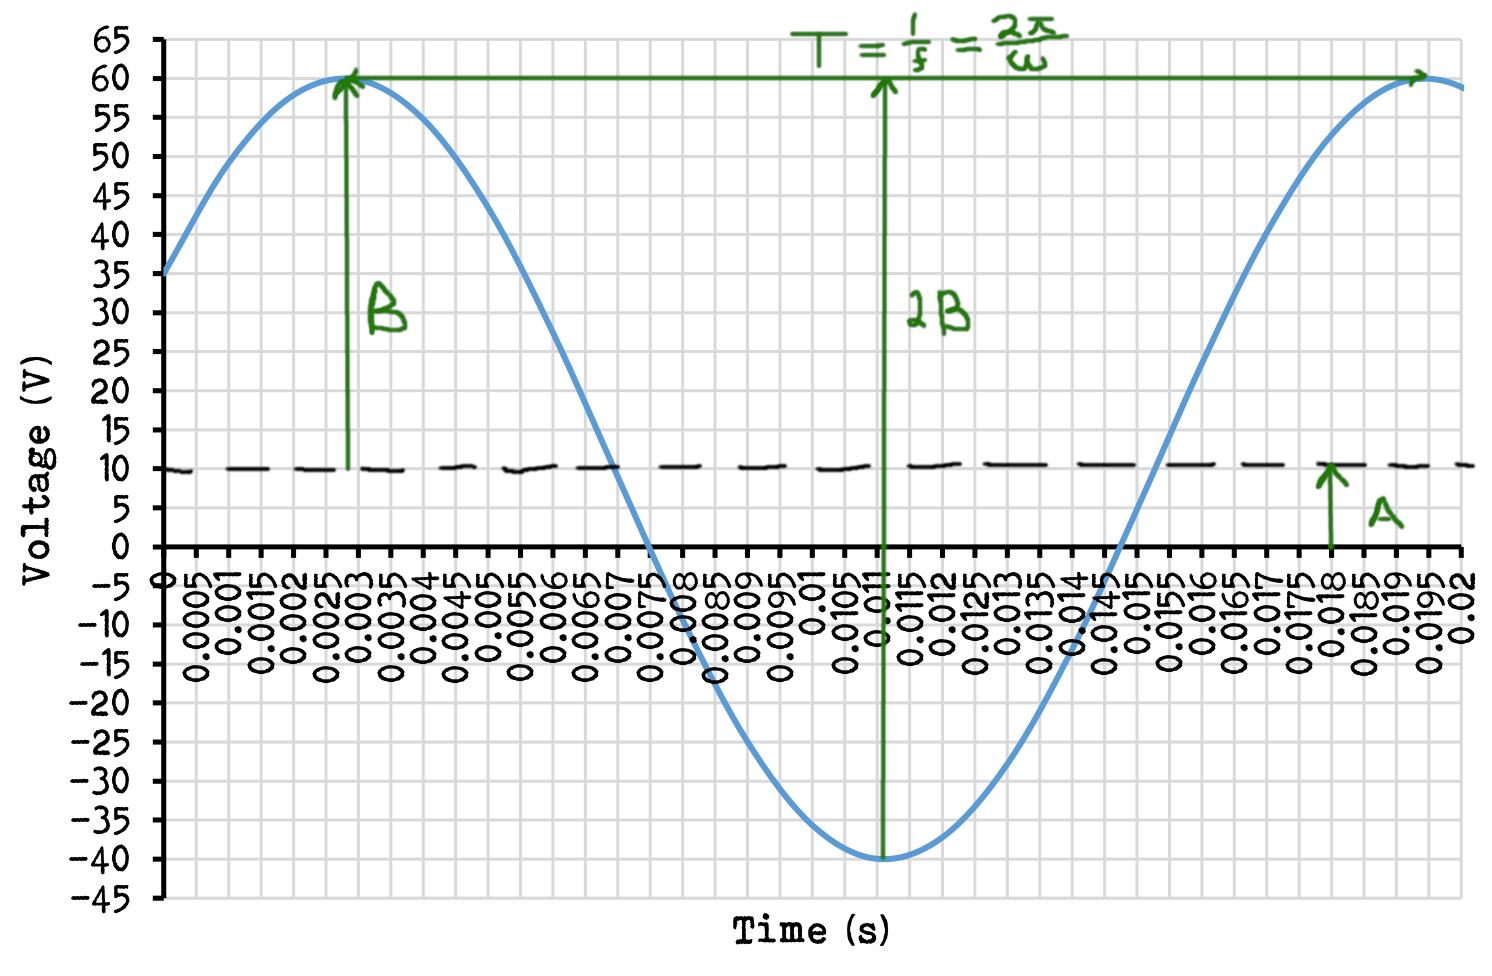
\includegraphics[width=\textwidth]{figure}
\begin{addmargin}[1.5cm]{0em}
	\noindent\textbf{Note:}
	\begin{equation}
		v(t) = \text{A} + \text{B} sin(\omega t + \Phi)
	\end{equation}
	\[ max_V = 60 \text{V} \]
	\[ min_V = -40 \text{V} \]
	\[ v(0) = 35 \text{V} \]
	\noindent\textbf{Assumptions:}
	\[ t_1 = 0.003 \text{s} \]
	\[ t_2 = 0.0195 \text{s} \]
	Its unclear where the peaks are exactly. \\
	\noindent\textbf{Solution:}
	\begingroup
	\allowdisplaybreaks
	\begin{align*}
		\text{Determine B} \\
		\text{B} &= {max_V - min_V \over 2} \\
		         &= {60 \text{V} - (-40 \text{V}) \over 2} \\
		         &= 50 \text{V} \\
		\text{Determine A} \\
		\text{A} &= {max_V + min_V \over 2} \\
		         &= {60 \text{V} - 40 \text{V} \over 2} \\
		         &= 10 \text{V} \\
		\text{Determin T} \\
		\text{T} &= t_2 - t_1 \\
		         &= 0.0195 \text{s} - 0.003 \text{s} \\
		         &= 0.0165 \text{s} \\
		\text{Determin $\Phi$} \\
		    v(t) &= \text{A} + \text{B} sin(\omega t + \Phi) \\
		{v(t) - \text{A} \over \text{B} } &= sin(\omega t + \Phi) \\
		\omega t + \Phi &= sin^{-1}({v(t) - \text{A} \over \text{B} }) \\
		    \Phi &= sin^{-1}({v(t) - \text{A} \over \text{B} }) - \omega t \\
		         &= sin^{-1}({35 \text{V} - 10 \text{V} \over 50 \text{V}}) - 380.8 \text{rad} / \text{s} \cdot 0 \text{s} \\
		         &= sin^{-1}({1 \over 2}) \\
		         &= {\pi \over 6} \\
	\end{align*}
	\endgroup
	\noindent\textbf{Answer:}
	\begin{itemize}
		\item A = 10 V
		\item B = 50 V
		\item T = 0.065 s
		\item $\Phi = {\pi \over 6}$
	\end{itemize}
\end{addmargin}
\newpage
\section{References}
[1] Denise Thorsen, Maher Al-Badri, INTRODUCTION TO ELECTRICAL AND COMPUTER ENGINEERING, University of Alaska Fairbanks, 2022.

\end{document}